\chapter{VolWeb: La Piattaforma Web per Volatility}

L'evoluzione degli strumenti di digital forensics ha sempre seguito un percorso che bilancia potenza analitica e accessibilità. In questo contesto, VolWeb emerge come una soluzione innovativa che affronta una delle sfide più significative nell'adozione della memory forensics: la complessità d'uso degli strumenti esistenti. Sviluppato come progetto open source, VolWeb si propone di rendere le capacità avanzate di Volatility 3 accessibili attraverso un'interfaccia web moderna, eliminando molte delle barriere che tradizionalmente hanno limitato l'adozione di queste tecniche investigative.

Il presente capitolo analizza in dettaglio l'architettura e le funzionalità della versione originale di VolWeb, fornendo il contesto necessario per comprendere le estensioni sviluppate in questa tesi. L'analisi si concentra sugli aspetti tecnici dell'implementazione, sulle scelte architetturali e sulle capacità forensi offerte dalla piattaforma.

\section{Genesi e Motivazioni del Progetto}

\subsection{Il contesto di sviluppo}

VolWeb \cite{volweb2024} nasce dalla constatazione di un paradosso nel campo della memory forensics: mentre Volatility si è affermato come lo standard per l'analisi della memoria, la sua adozione rimane limitata a specialisti con competenze tecniche avanzate. Questa situazione crea un collo di bottiglia operativo in molte organizzazioni, dove la capacità di analizzare rapidamente dump di memoria può fare la differenza tra contenere un incidente o subirne le conseguenze complete.

Il progetto, avviato nel 2023, si inserisce in un momento storico particolare per la cybersecurity. L'aumento esponenziale degli attacchi ransomware, la sofisticazione crescente delle Advanced Persistent Threats e l'adozione massiva del lavoro remoto hanno moltiplicato la superficie di attacco delle organizzazioni. In questo scenario, la capacità di condurre analisi forensi rapide ed efficaci diventa non più un lusso per pochi specialisti, ma una necessità operativa diffusa.

Come descritto nella documentazione ufficiale del progetto, VolWeb è "a digital forensic memory analysis platform that leverages the power of the Volatility 3 framework". Questa definizione sintetica cattura l'essenza del progetto: non un sostituto di Volatility, ma un amplificatore delle sue capacità attraverso un'interfaccia che ne democratizza l'accesso.

\subsection{Obiettivi progettuali}

L'obiettivo primario di VolWeb è la democratizzazione dell'accesso alle capacità di memory forensics. Questo si traduce concretamente nel fornire un'interfaccia che nasconda la complessità di Volatility senza sacrificarne la potenza. Il progetto mira a ridurre il tempo necessario per ottenere risultati actionable da ore a minuti, permettendo anche ad analisti con esperienza limitata di condurre investigazioni efficaci.

Un secondo obiettivo fondamentale riguarda la standardizzazione dei workflow investigativi. Mentre l'uso diretto di Volatility lascia ampia libertà nell'approccio all'analisi, questa flessibilità può tradursi in inconsistenza e inefficienza, specialmente in team con membri di diversa esperienza. VolWeb introduce un framework strutturato che guida l'analista attraverso le fasi dell'investigazione, garantendo completezza e riproducibilità.

La collaborazione rappresenta il terzo pilastro degli obiettivi progettuali. Le investigazioni moderne raramente coinvolgono un singolo analista; più spesso richiedono il coordinamento di team distribuiti geograficamente e temporalmente. VolWeb fornisce un ambiente condiviso dove più analisti possono lavorare sugli stessi casi, condividere osservazioni e costruire collettivamente la comprensione di un incidente.

\section{Requisiti di Sistema e Installazione}

\subsection{Prerequisiti}

Prima di procedere con l'installazione di VolWeb, è necessario verificare che l'ambiente soddisfi i requisiti minimi. Il sistema richiede Python 3.8 o superiore, fondamentale per la compatibilità con Volatility 3 e le librerie moderne utilizzate. È inoltre necessario avere Git installato per clonare il repository e Docker con Docker Compose per il deployment containerizzato, che rappresenta il metodo di installazione raccomandato.

Dal punto di vista hardware, sebbene VolWeb possa funzionare su sistemi modesti per analisi di piccola scala, per un utilizzo produttivo si raccomandano almeno 8 GB di RAM e storage sufficiente per i dump di memoria, che possono facilmente raggiungere decine di gigabyte per sistema analizzato.

\subsection{Processo di installazione}

L'installazione di VolWeb è stata progettata per essere il più semplice possibile, riconoscendo che la complessità di setup è spesso una barriera all'adozione. Il processo standard prevede prima di tutto la clonazione del repository:

\begin{minted}[bgcolor=gray!10, fontsize=\small]{bash}
git clone https://github.com/k1nd0ne/VolWeb.git
cd VolWeb
\end{minted}

Successivamente, l'ambiente può essere avviato utilizzando Docker Compose, che gestisce automaticamente tutte le dipendenze e configurazioni:

\begin{minted}[bgcolor=gray!10, fontsize=\small]{bash}
docker-compose up -d
\end{minted}

Questo comando avvia tutti i servizi necessari: il backend Django, il frontend React, PostgreSQL per la persistenza dei dati, Redis per il caching e message brokering, e i Celery workers per l'elaborazione asincrona.

Per ambienti di sviluppo o per chi preferisce un'installazione manuale, VolWeb supporta anche il setup tradizionale. Questo richiede l'installazione separata delle dipendenze Python tramite pip, la configurazione del database PostgreSQL, l'avvio di Redis e la configurazione manuale delle variabili d'ambiente. Sebbene più complesso, questo approccio offre maggiore controllo e facilita il debugging durante lo sviluppo.

\section{Architettura del Sistema}

\subsection{Principi architetturali}

L'architettura di VolWeb riflette una filosofia di design che privilegia modularità, estensibilità e manutenibilità. La scelta di un'architettura web-based non è casuale, ma deriva da considerazioni pratiche sull'uso reale dello strumento in contesti operativi. Gli analisti forensi operano spesso in condizioni di emergenza, da postazioni diverse e con risorse hardware variabili. Un'applicazione web elimina le frizioni legate all'installazione e configurazione di software complesso, permettendo un accesso immediato alle funzionalità di analisi.

La separazione tra frontend e backend attraverso API REST \cite{restapi} rappresenta una scelta architettonica fondamentale che va oltre la semplice modularizzazione del codice. Questa separazione permette l'evoluzione indipendente dei componenti, facilitando sia lo sviluppo che la manutenzione. Inoltre, esporre le funzionalità attraverso API standardizzate apre la possibilità di integrazioni con altri strumenti dell'ecosistema di sicurezza, trasformando VolWeb da applicazione standalone a componente di pipeline di analisi più ampie.

\subsection{Stack tecnologico}

\begin{figure}[H]
    \centering   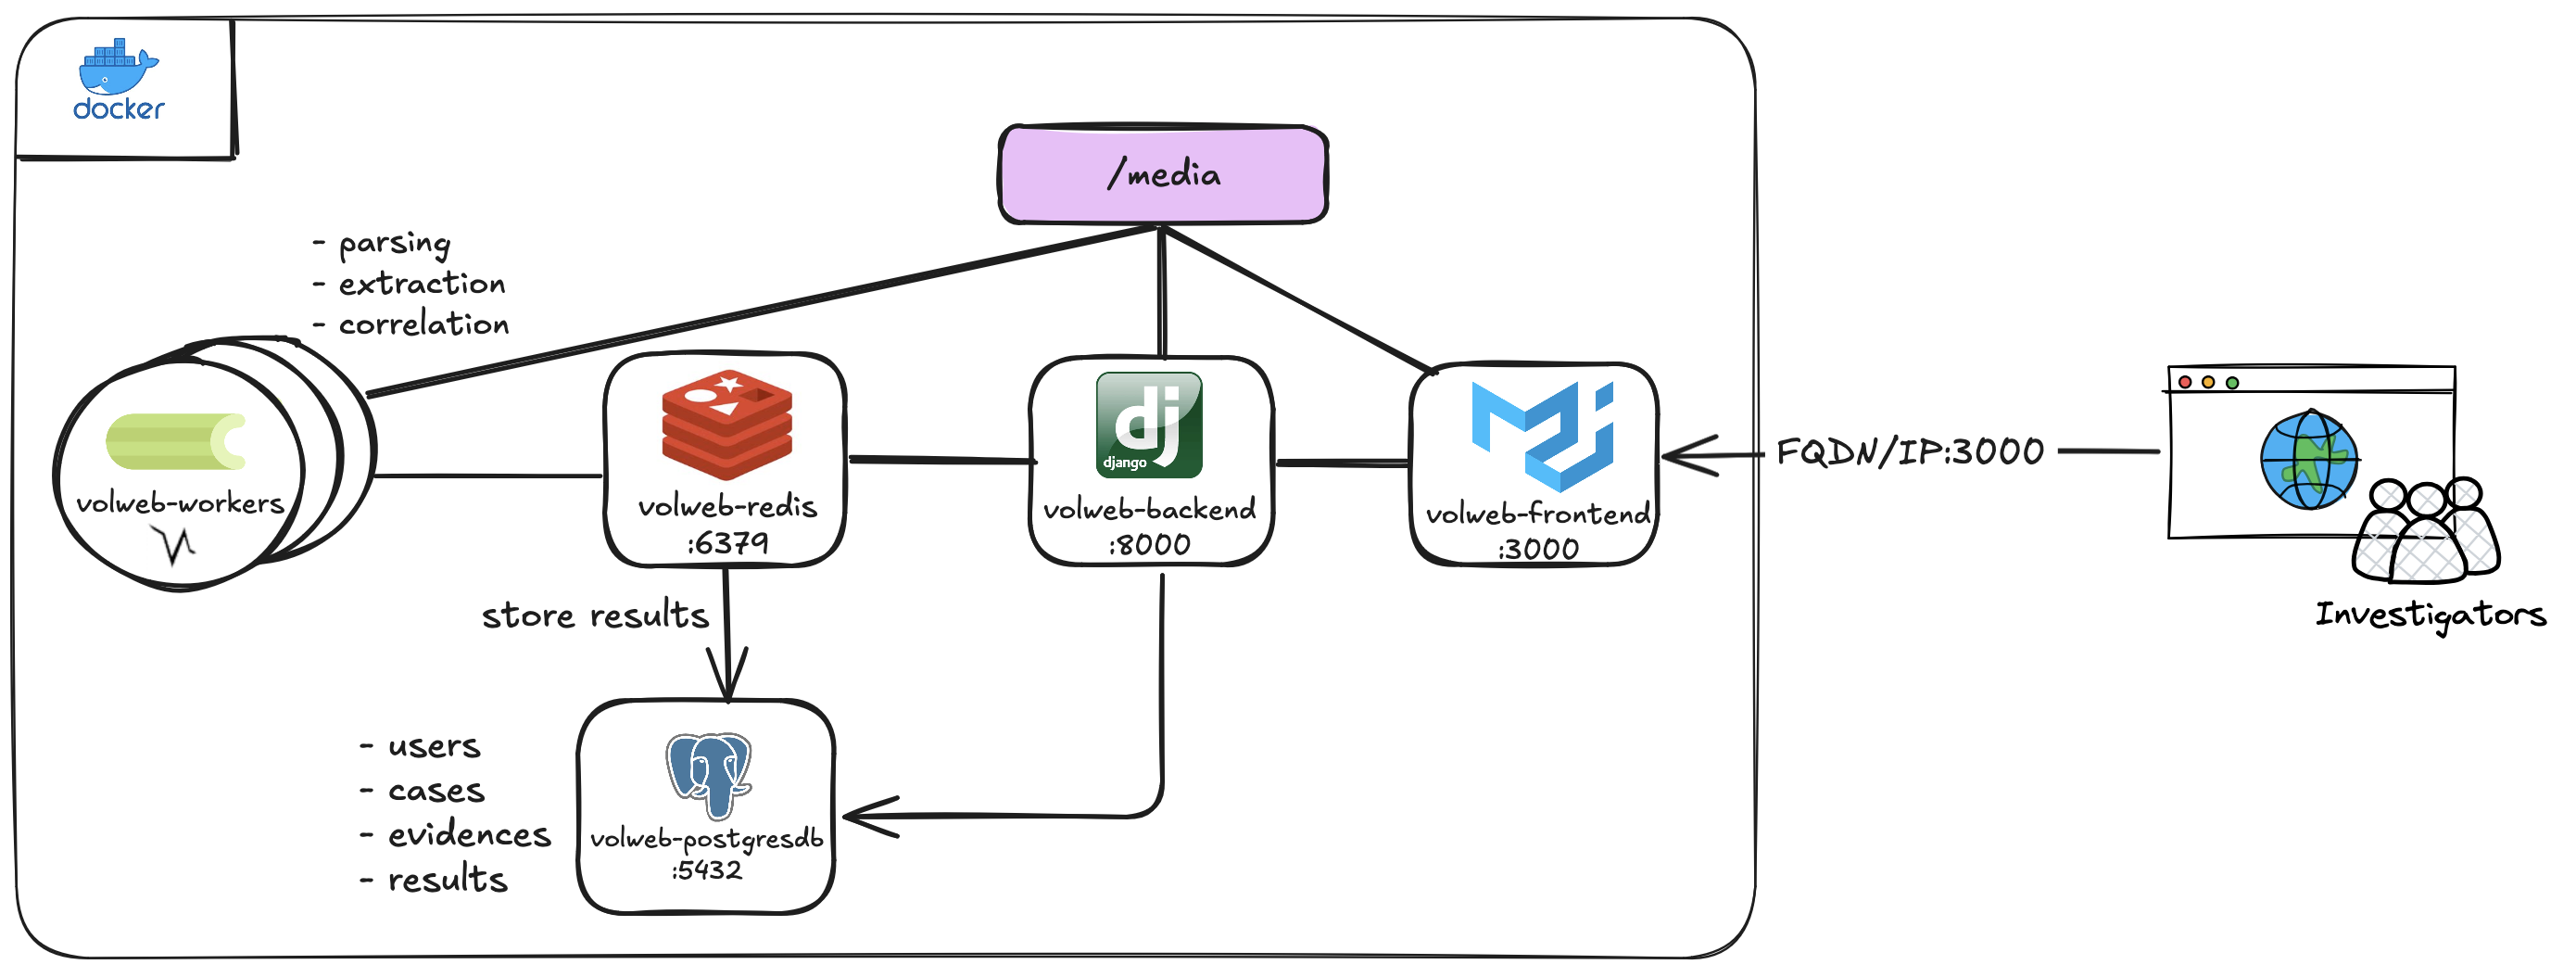
\includegraphics[width=1\linewidth]{images/volweb-original/volweb-arch.png}
\end{figure}

La selezione delle tecnologie utilizzate in VolWeb riflette un bilanciamento tra maturità, performance e facilità di sviluppo. Il backend, costruito su Django 4.2 e Django REST Framework, sfrutta un ecosistema consolidato che offre soluzioni robuste per problematiche comuni come autenticazione, gestione delle sessioni e validazione dei dati.

Il frontend utilizza React 18.2.0 con Material-UI 5.14 per l'interfaccia utente. Questa combinazione fornisce un'esperienza utente moderna e reattiva, fondamentale per mantenere l'efficienza operativa durante investigazioni che possono protrarsi per ore. La scelta di Material-UI come design system garantisce consistenza visiva e accessibilità, aspetti spesso trascurati nei tool forensi ma cruciali per ridurre il carico cognitivo dell'analista.

Per la gestione dei task asincroni, VolWeb si affida a Celery 5.3 con Redis come message broker. Questa architettura permette di gestire operazioni computazionalmente intensive come l'analisi di dump di memoria di grandi dimensioni senza bloccare l'interfaccia utente. La scalabilità orizzontale offerta da Celery consente inoltre di distribuire il carico di lavoro su molteplici macchine, aspetto critico quando si devono analizzare contemporaneamente dump provenienti da decine di endpoint compromessi.

La persistenza dei dati è affidata a PostgreSQL, scelto per la sua affidabilità e le capacità avanzate di gestione di dati JSON, particolarmente utili per memorizzare i risultati strutturati ma eterogenei prodotti dai vari plugin di Volatility. L'uso di SQLite come alternativa per deployment di sviluppo o di piccola scala dimostra l'attenzione alla flessibilità di deployment.

\subsection{Integrazione con Volatility 3}

Il cuore tecnico di VolWeb risiede nell'integrazione con Volatility 3, realizzata attraverso un layer di astrazione che gestisce la complessità dell'interazione con il framework. Questa integrazione non si limita a un semplice wrapper delle funzionalità command-line, ma implementa una gestione sofisticata del ciclo di vita dell'analisi.

Il modulo definito in 'backend/volatility\_engine.py', implementa un'interfaccia Python nativa con Volatility 3. Questo approccio elimina l'overhead dell'invocazione di processi esterni e permette un controllo granulare sull'esecuzione dei plugin. La gestione della configurazione di Volatility, tradizionalmente complessa e error-prone, viene automatizzata attraverso la costruzione dinamica del contesto di esecuzione basata sui metadati del dump analizzato.

Un aspetto particolarmente innovativo dell'integrazione riguarda la gestione dei simboli. Volatility richiede symbol tables specifiche per ogni versione di sistema operativo per interpretare correttamente le strutture dati in memoria. VolWeb automatizza il download e la gestione di questi simboli, eliminando uno dei principali ostacoli tecnici nell'uso di Volatility. Il sistema mantiene una cache locale dei simboli più comuni e scarica automaticamente quelli mancanti quando necessario. Inoltre, permette anche di caricare manualmente i file dei simboli direttamente dal file system, offrendo all'utente un controllo completo in caso di configurazioni particolari o ambienti offline.

La gestione degli errori rappresenta un altro aspetto critico dell'integrazione. I plugin di Volatility possono fallire per molteplici ragioni, dalla corruzione del dump all'incompatibilità con la versione del sistema operativo. VolWeb implementa una strategia di error handling che distingue tra errori fatali e warning, permettendo all'analisi di procedere anche quando singoli plugin falliscono, mentre registra dettagliatamente le cause del fallimento per troubleshooting successivo.

\section{Workflow Operativo e Funzionalità}

\subsection{Gestione dei casi}

Il workflow operativo di VolWeb inizia con la creazione di un caso, che rappresenta il contenitore logico per un'investigazione. Ogni caso può aggregare molteplici evidenze, permettendo l'analisi correlata di dump provenienti da sistemi diversi coinvolti nello stesso incidente. La gestione dei casi segue best practice forensi, mantenendo metadati completi su chi ha creato il caso, quando è stato modificato e quale sia il suo stato corrente.

\begin{figure}[H]
    \centering
    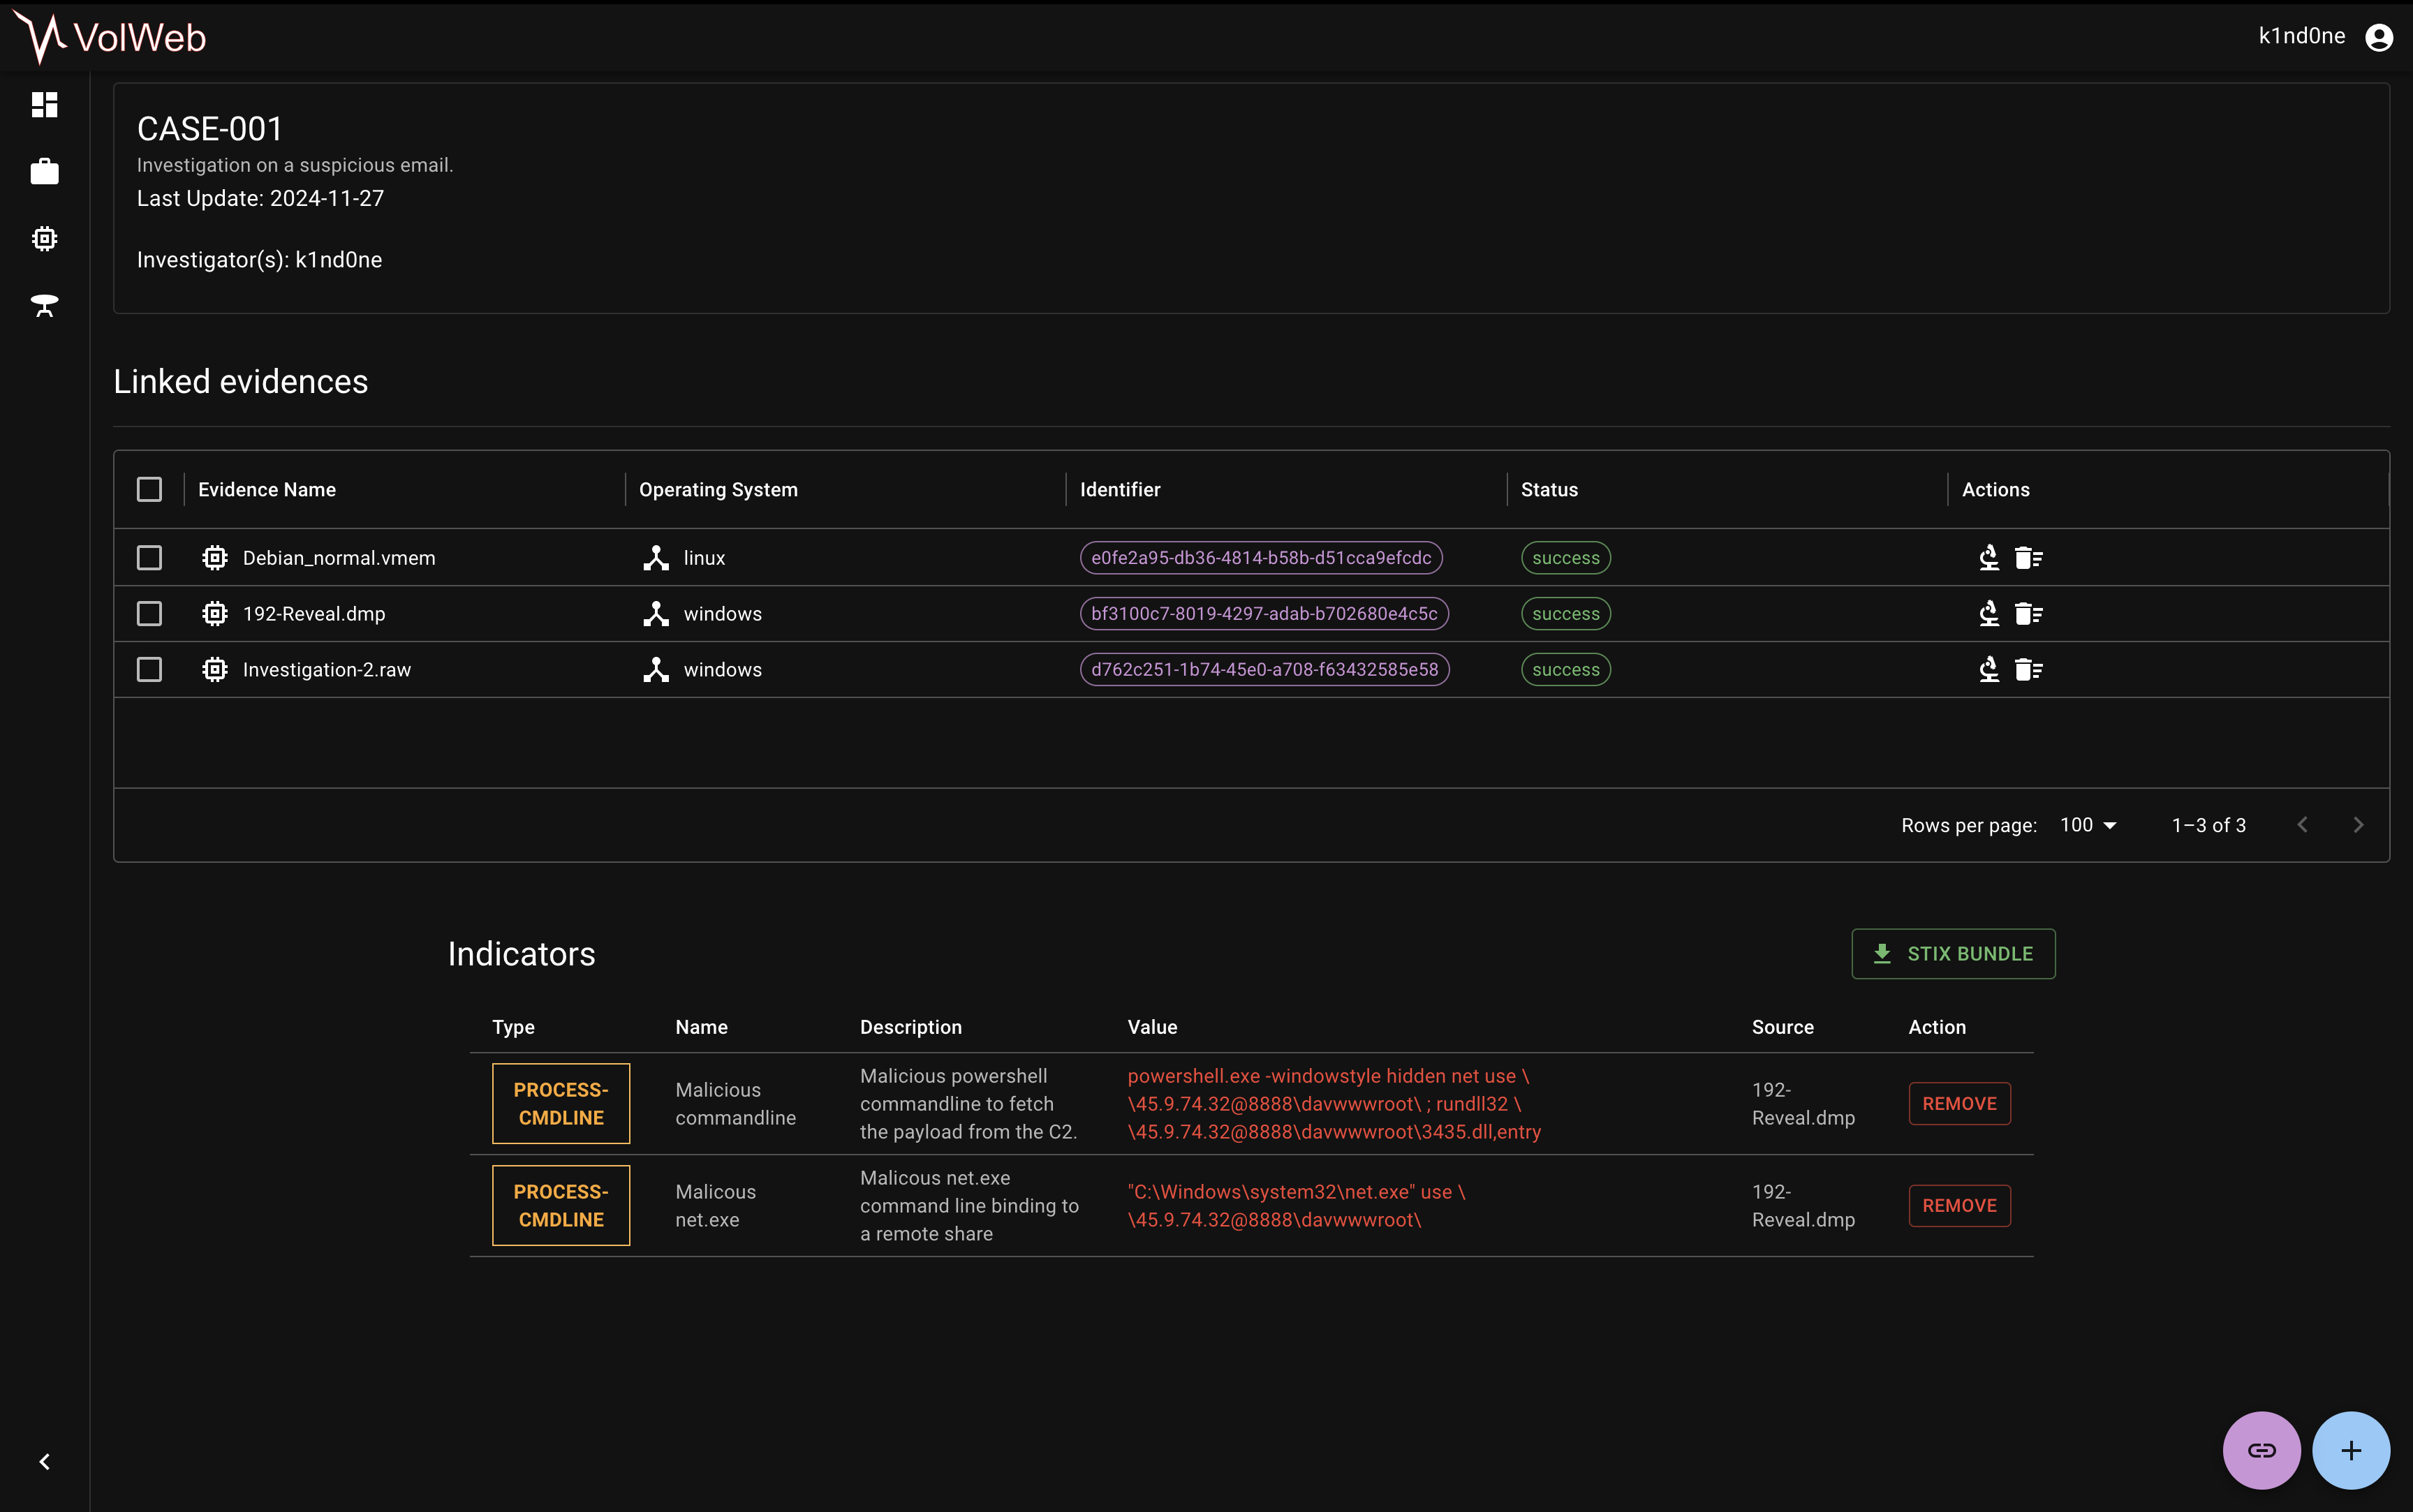
\includegraphics[width=1\linewidth]{images/volweb-original/volweb-case-management.png}
\end{figure}

L'interfaccia di gestione dei casi presenta una dashboard che fornisce una vista immediata dello stato delle investigazioni. Ogni caso è rappresentato da una card che mostra informazioni essenziali: nome, descrizione, numero di evidenze associate, stato dell'analisi e ultima modifica. Questa presentazione visiva permette agli analisti di prioritizzare rapidamente il proprio lavoro e identificare casi che richiedono attenzione immediata.

\subsection{Upload e gestione delle evidenze}

Una volta creato un caso, il passo successivo è l'upload dei dump di memoria da analizzare. VolWeb gestisce questo processo critico con particolare attenzione all'integrità dei dati e all'esperienza utente. L'interfaccia di upload supporta drag-and-drop, permettendo agli utenti di trascinare file direttamente dal file manager del sistema operativo.

\begin{figure}[H]
    \centering
    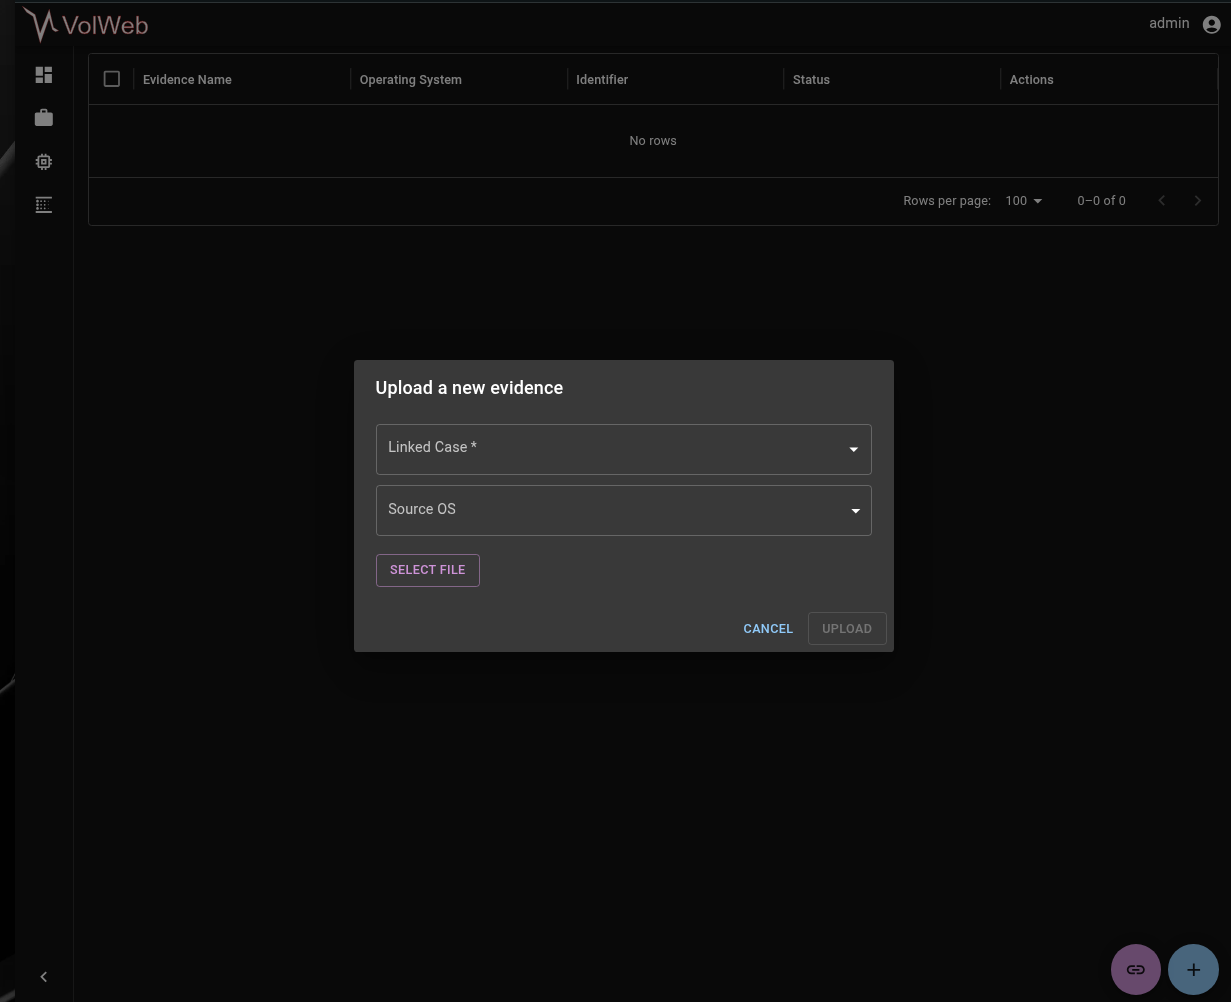
\includegraphics[width=0.9\linewidth]{images/volweb-original/volweb-upload-interface.png}
\end{figure}

Per file di grandi dimensioni, comune scenario con dump di memoria che possono superare i 16GB, VolWeb implementa un sistema di upload chunked. Questo approccio divide il file in blocchi più piccoli che vengono trasmessi sequenzialmente, con la possibilità di riprendere l'upload in caso di interruzione della connessione.

\subsection{Analisi automatica}

Dopo il completamento dell'upload, VolWeb avvia automaticamente una serie di analisi predefinite progettate per fornire una panoramica immediata del sistema analizzato. Questa suite di plugin include l'enumerazione dei processi (pslist), l'analisi delle connessioni di rete (netscan), l'estrazione delle command line (cmdline), la lista delle DLL caricate (dlllist) e l'identificazione degli handle aperti (handles).

La selezione di questi plugin non è casuale ma deriva dall'esperienza operativa che identifica queste informazioni come il minimo dataset necessario per una comprensione iniziale dello stato del sistema. L'esecuzione automatica elimina la necessità per l'analista di ricordare quali plugin eseguire per primi, standardizzando l'approccio investigativo.

Durante l'analisi, VolWeb fornisce feedback dettagliato attraverso WebSocket, mostrando quale plugin è in esecuzione, la percentuale di completamento e eventuali warning o errori. Questo feedback real-time è cruciale per mantenere la fiducia dell'utente durante operazioni che possono richiedere tempo significativo.

\subsection{Visualizzazione e esplorazione dei risultati}

La presentazione efficace dei risultati rappresenta uno dei maggiori valori aggiunti di VolWeb rispetto all'uso diretto di Volatility. Invece di output testuali densi, VolWeb trasforma i dati in visualizzazioni interattive che facilitano l'identificazione di anomalie e pattern sospetti.

\begin{figure}[H]
    \centering
    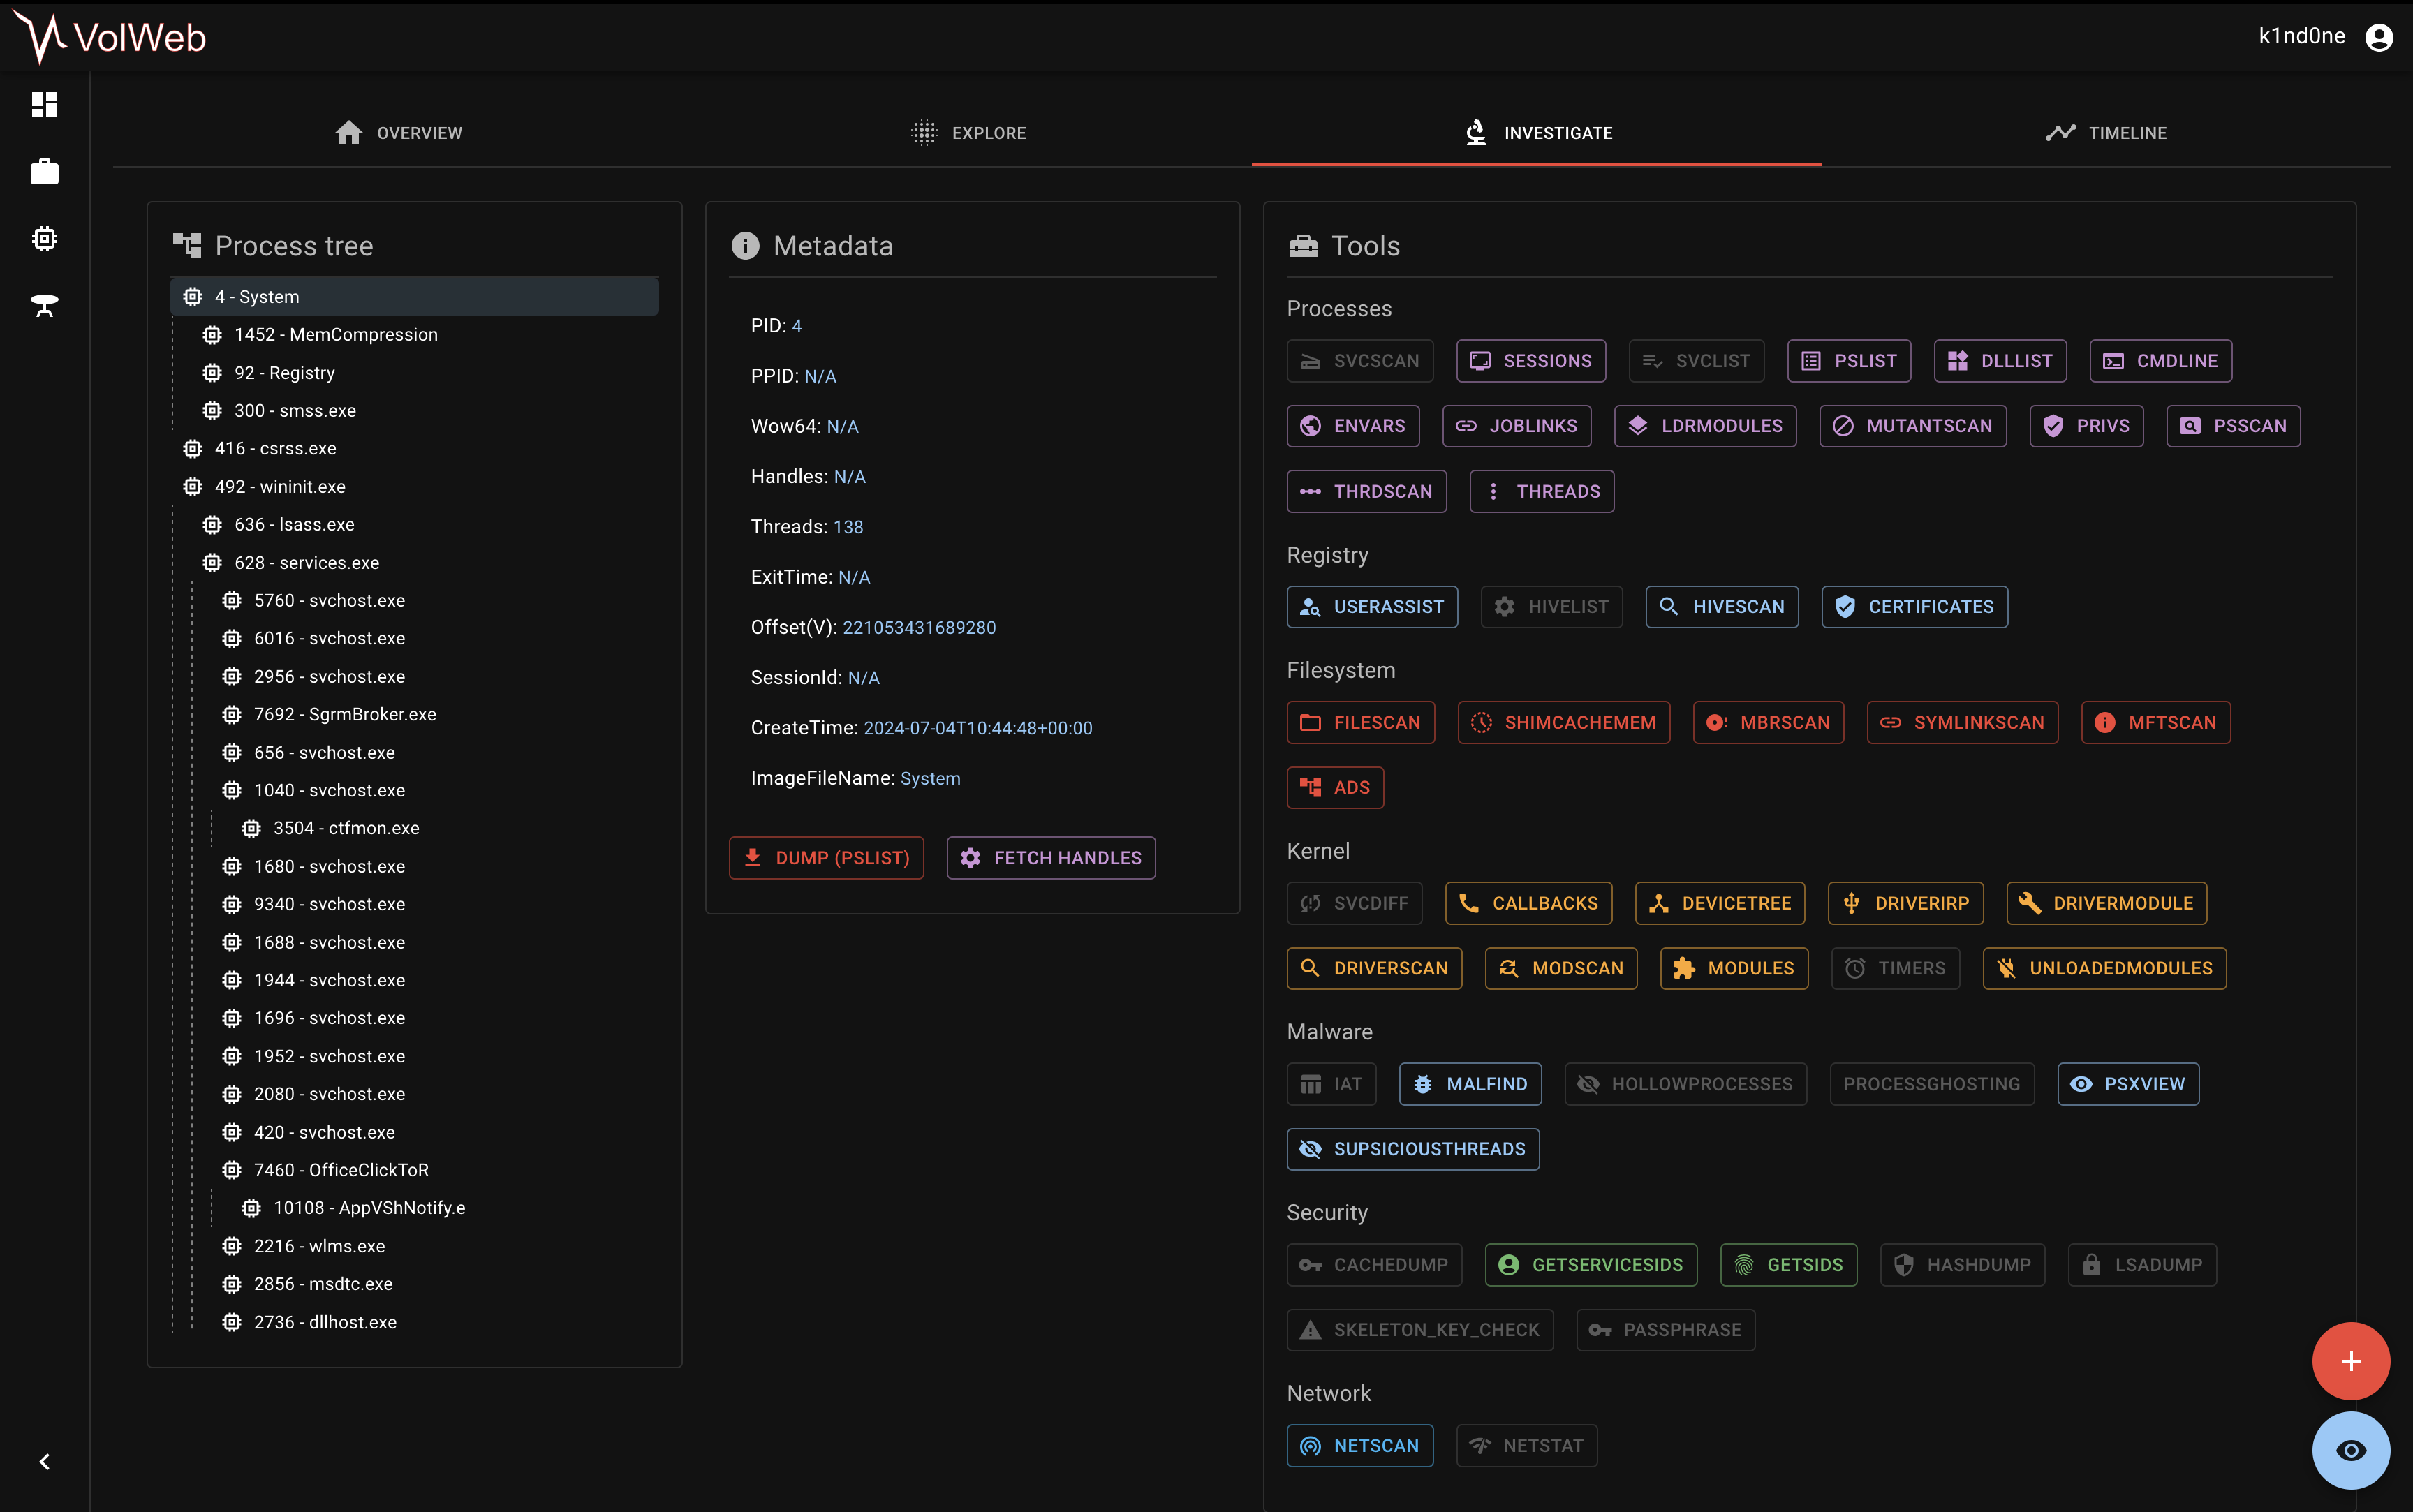
\includegraphics[width=1\linewidth]{images/volweb-original/volweb-process-tree.png}
\end{figure}

La vista dei processi utilizza una rappresentazione ad albero che mostra chiaramente le relazioni parent-child tra processi. I processi orfani o con parent inusuali sono evidenziati visivamente, permettendo l'identificazione rapida di potenziali indicatori di compromissione. Ogni nodo dell'albero è espandibile per rivelare dettagli aggiuntivi: PID, tempo di creazione, numero di thread e handle, spazio di memoria utilizzato.

Per le connessioni di rete, VolWeb offre multiple viste complementari. La vista tabellare fornisce tutti i dettagli tecnici: processo proprietario, protocollo, indirizzi IP e porte locali e remote, stato della connessione. La vista grafica, basata su D3.js, visualizza le connessioni come un grafo interattivo dove i nodi rappresentano processi ed endpoint, mentre gli archi indicano le connessioni attive.

\begin{figure}[H]
    \centering
    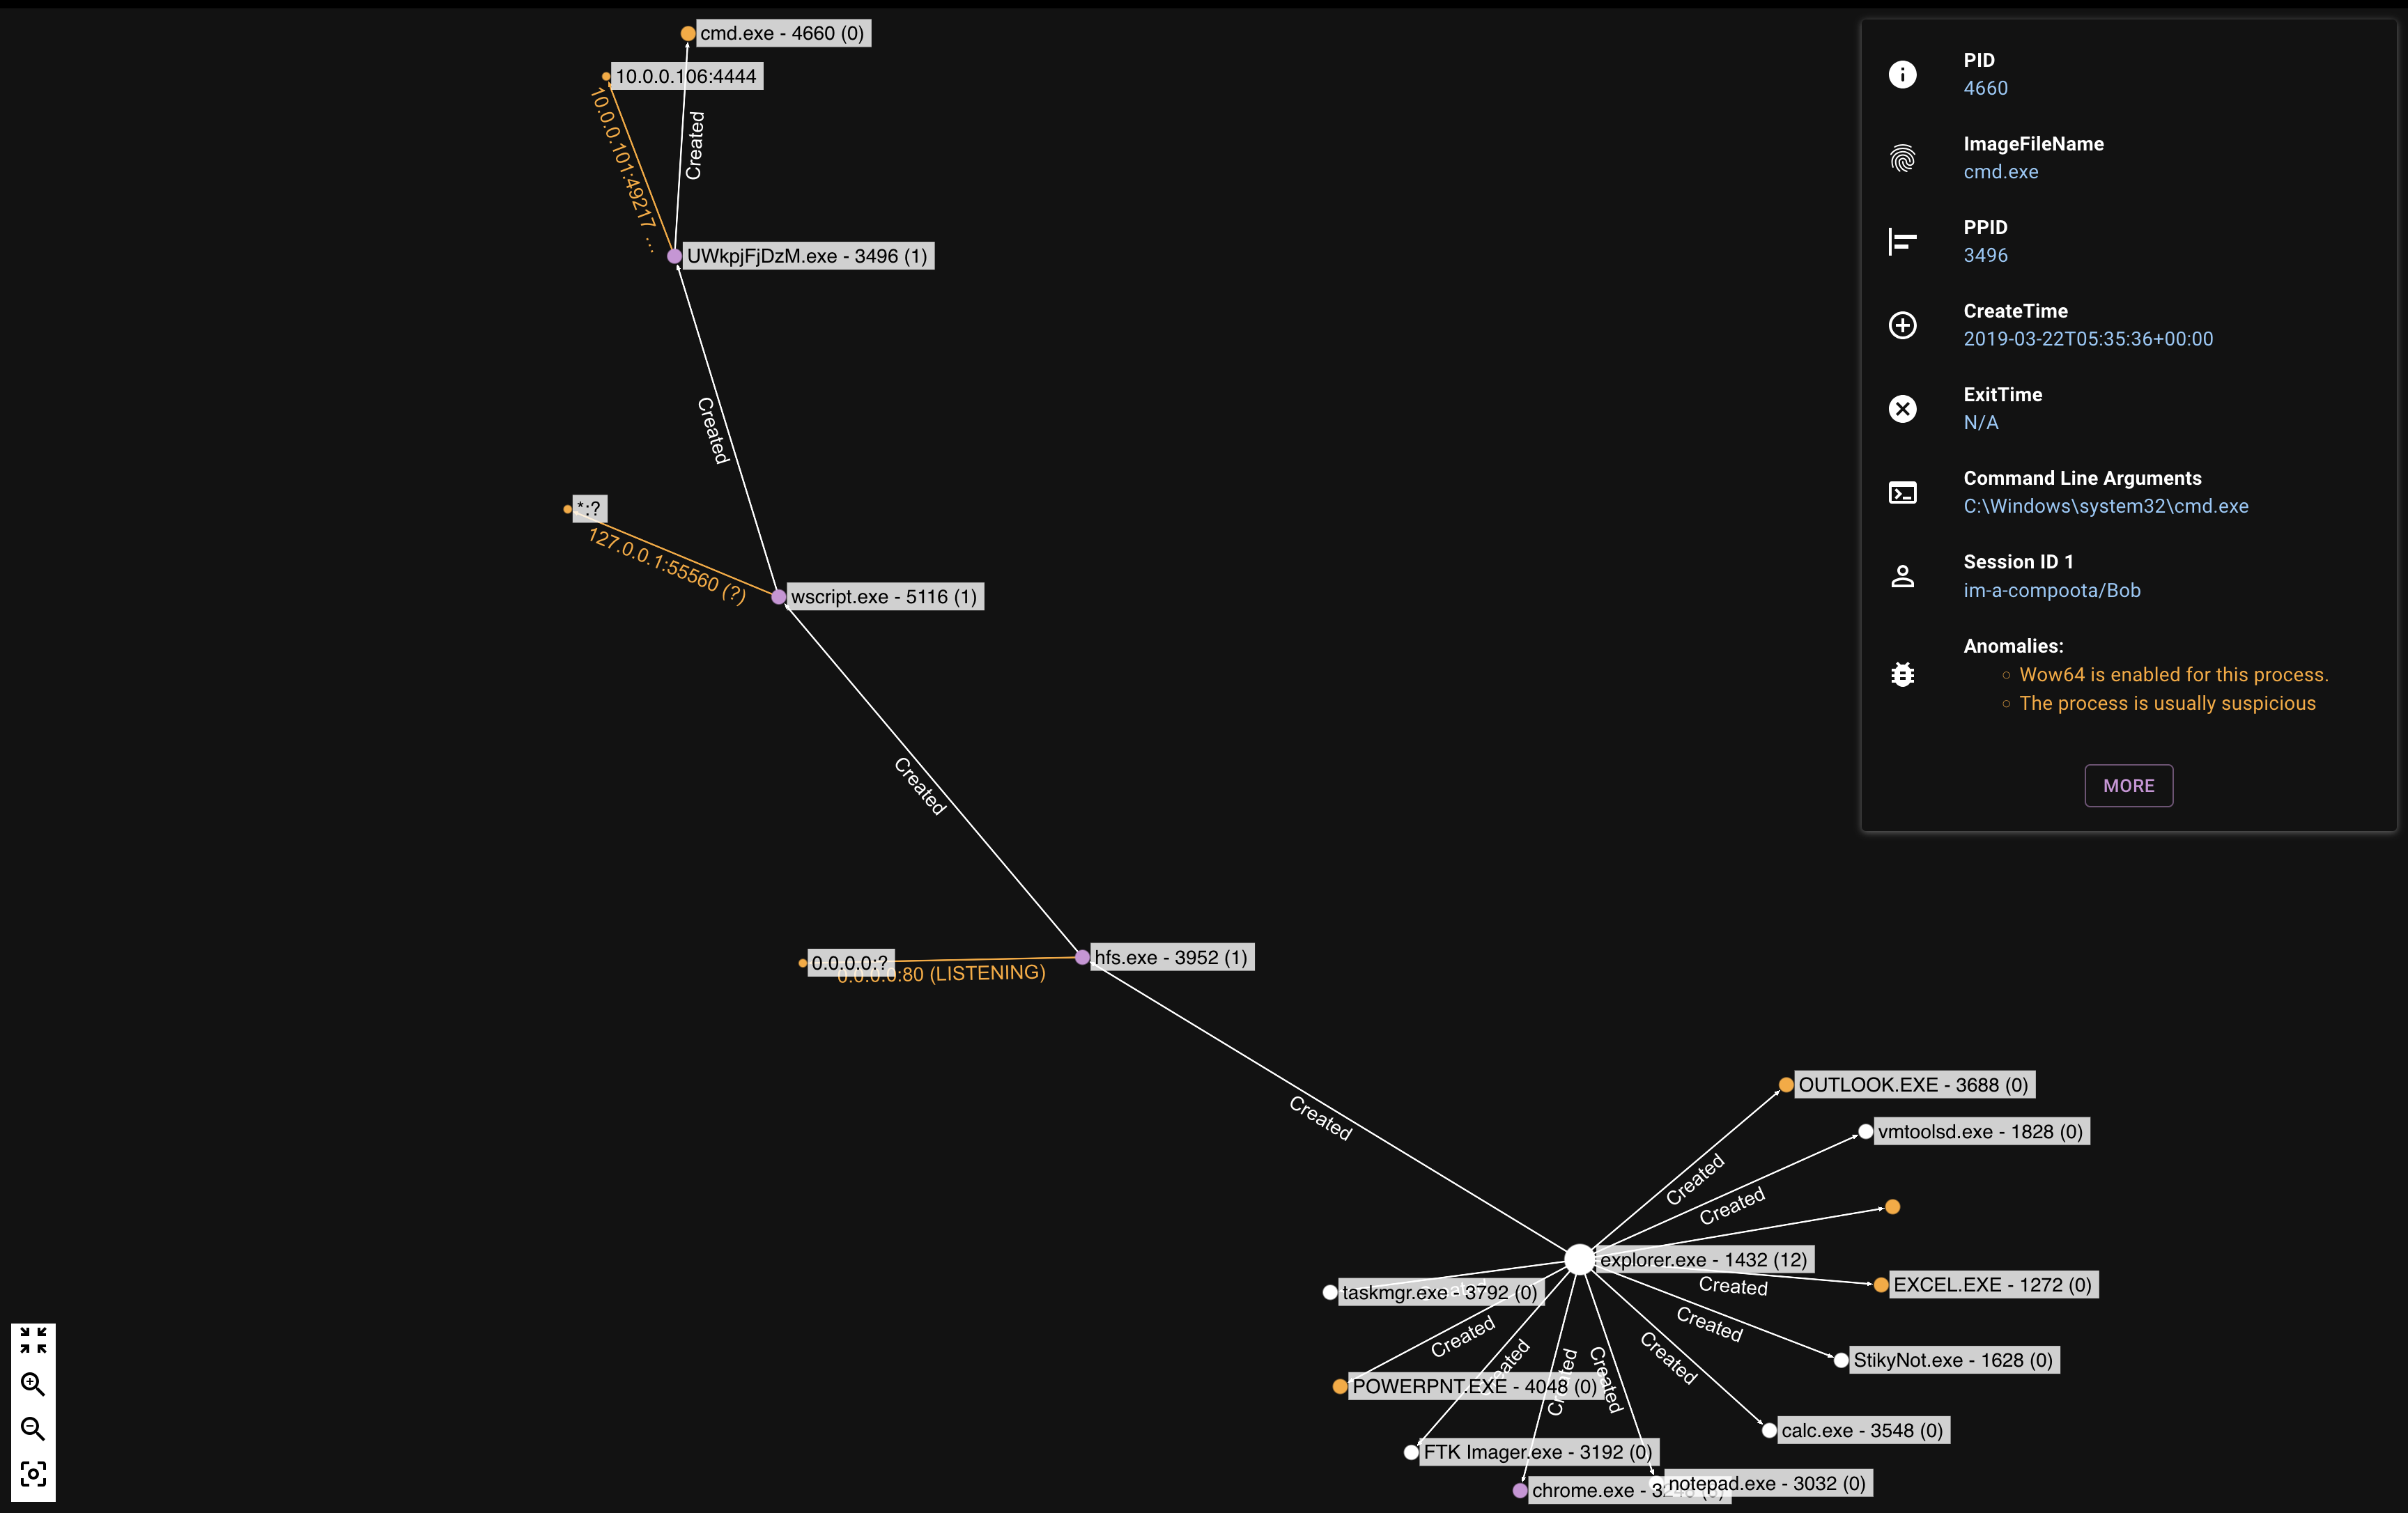
\includegraphics[width=0.9\linewidth]{images/volweb-original/volweb-network-graph.png}
\end{figure}

\subsection{Ricerca e filtering avanzati}

Con dump di memoria che possono contenere informazioni su centinaia di processi e migliaia di artefatti, la capacità di ricerca efficace diventa critica. VolWeb implementa un motore di ricerca che supporta query sia semplici che complesse, permettendo agli analisti di trovare rapidamente informazioni rilevanti.

La ricerca full-text opera su tutti i campi dei risultati, permettendo di trovare rapidamente riferimenti a file specifici, indirizzi IP, o stringhe sospette. Il sistema supporta inoltre filtering avanzato per tipo di dato, permettendo per esempio di visualizzare solo i processi che hanno connessioni di rete attive o solo le DLL caricate da percorsi non standard.

\section{Interfaccia Utente e User Experience}

\subsection{Design dell'interfaccia}

L'interfaccia di VolWeb rappresenta un `departure` significativo dall'approccio command-line tradizionale di Volatility. Il design, basato sui principi del Material Design, prioritizza la chiarezza e l'efficienza operativa. La dashboard principale presenta una vista d'insieme dei casi attivi, permettendo all'analista di comprendere immediatamente lo stato delle investigazioni in corso.

\begin{figure}[H]
    \centering
    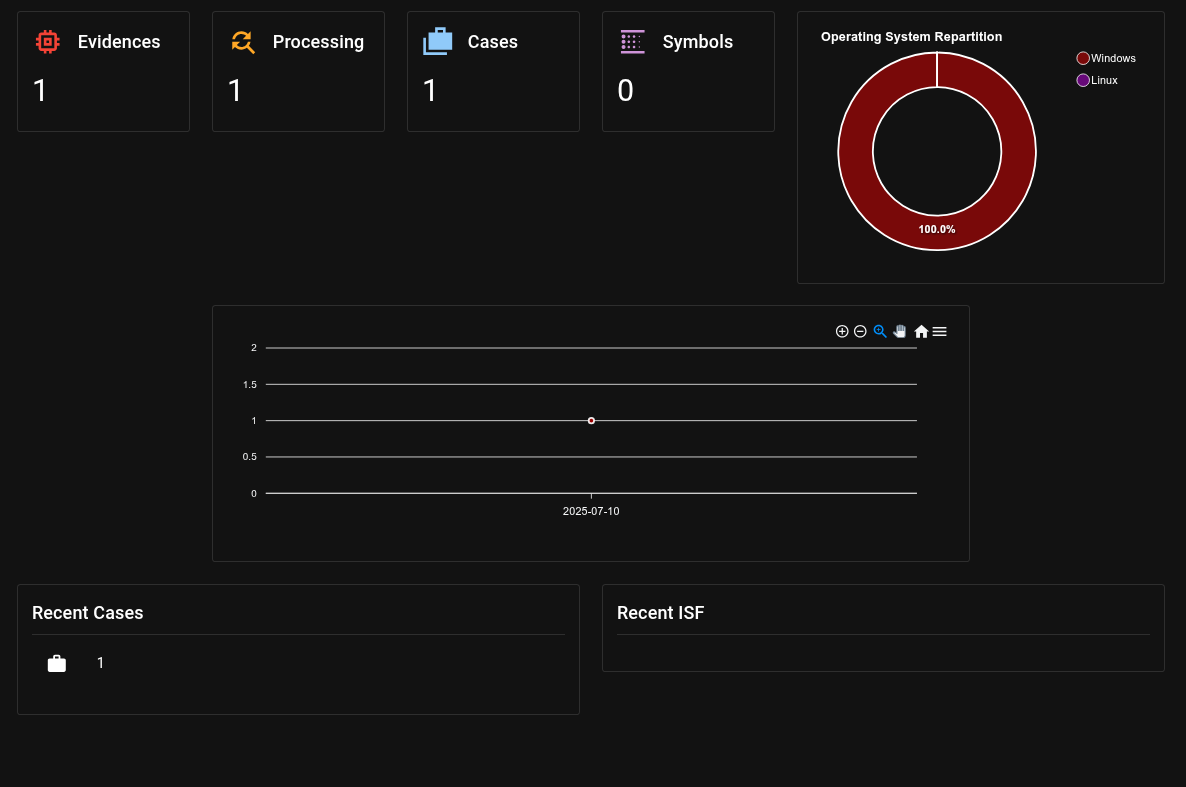
\includegraphics[width=1\linewidth]{images/volweb-original/volweb-dashboard.png}
\end{figure}

La navigazione segue una struttura gerarchica naturale: dalla lista dei casi si accede ai dettagli del singolo caso, da cui è possibile esplorare le evidenze associate e i risultati delle analisi. Questa struttura, apparentemente semplice, nasconde una considerevole complessità nell'orchestrazione dei componenti React che gestiscono lo stato dell'applicazione.

L'uso estensivo di feedback visivo mantiene l'utente informato sullo stato delle operazioni. Progress bar per upload e analisi, notifiche per il completamento di task e indicatori di stato per ogni componente contribuiscono a creare un'esperienza utente che minimizza l'incertezza e l'ansia tipiche delle operazioni di lunga durata.

\subsection{Visualizzazione dei risultati}

La presentazione dei risultati dell'analisi rappresenta una delle sfide principali nel design di VolWeb. I plugin di Volatility producono output eterogenei, da semplici liste a strutture dati complesse. VolWeb implementa renderer specializzati per i tipi di dati più comuni, trasformando tabelle di testo in visualizzazioni interattive.

Per i dati di processo, il sistema presenta una vista tabellare arricchita che permette sorting, filtering e ricerca full-text. Ogni processo è cliccabile per accedere a una vista dettagliata che aggrega informazioni da multipli plugin correlati. Questa aggregazione, invisibile all'utente, richiede una logica complessa per correlare dati provenienti da plugin diversi basandosi su identificatori comuni come PID e offset di memoria.

Le informazioni di rete sono presentate attraverso una combinazione di viste tabellari e visualizzazioni grafiche. La vista tabellare permette un'analisi dettagliata di ogni connessione, mentre la visualizzazione grafica offre una comprensione immediata delle relazioni tra processi e endpoint remoti.

\section{Sistema di Plugin e Estensibilità}

VolWeb implementa un sistema di plugin che riflette e estende quello di Volatility. Ogni plugin supportato è rappresentato da una configurazione che specifica parametri, dipendenze e modalità di visualizzazione dei risultati. Questa architettura permette di aggiungere supporto per nuovi plugin di Volatility senza modifiche al core dell'applicazione.

L'esecuzione dei plugin avviene attraverso Celery task che permettono parallelizzazione e gestione robusta degli errori. Quando un utente richiede l'esecuzione di un'analisi, VolWeb crea un task Celery per ogni plugin selezionato. Questi task vengono distribuiti ai worker disponibili, permettendo l'esecuzione parallela su hardware multi-core o distribuito.

L'orchestrazione dei plugin tiene conto delle dipendenze tra di essi. Alcuni plugin richiedono i risultati di altri per funzionare correttamente. VolWeb gestisce automaticamente queste dipendenze, assicurando che i plugin vengano eseguiti nell'ordine corretto e che i risultati siano disponibili quando necessario.

\section{API REST}

VolWeb espone una API REST completa che permette l'automazione e l'integrazione con altri strumenti. La documentazione delle API, generata automaticamente da Django REST Framework, fornisce dettagli su ogni endpoint disponibile, parametri richiesti e formato delle risposte.

Gli endpoint principali includono la gestione dei casi con creazione, modifica e cancellazione; la gestione delle evidenze con upload, download e metadata; l'esecuzione dei plugin con selezione, parametrizzazione e monitoraggio; il recupero dei risultati con filtering, paginazione ed export.

\begin{figure}[H]
    \centering
    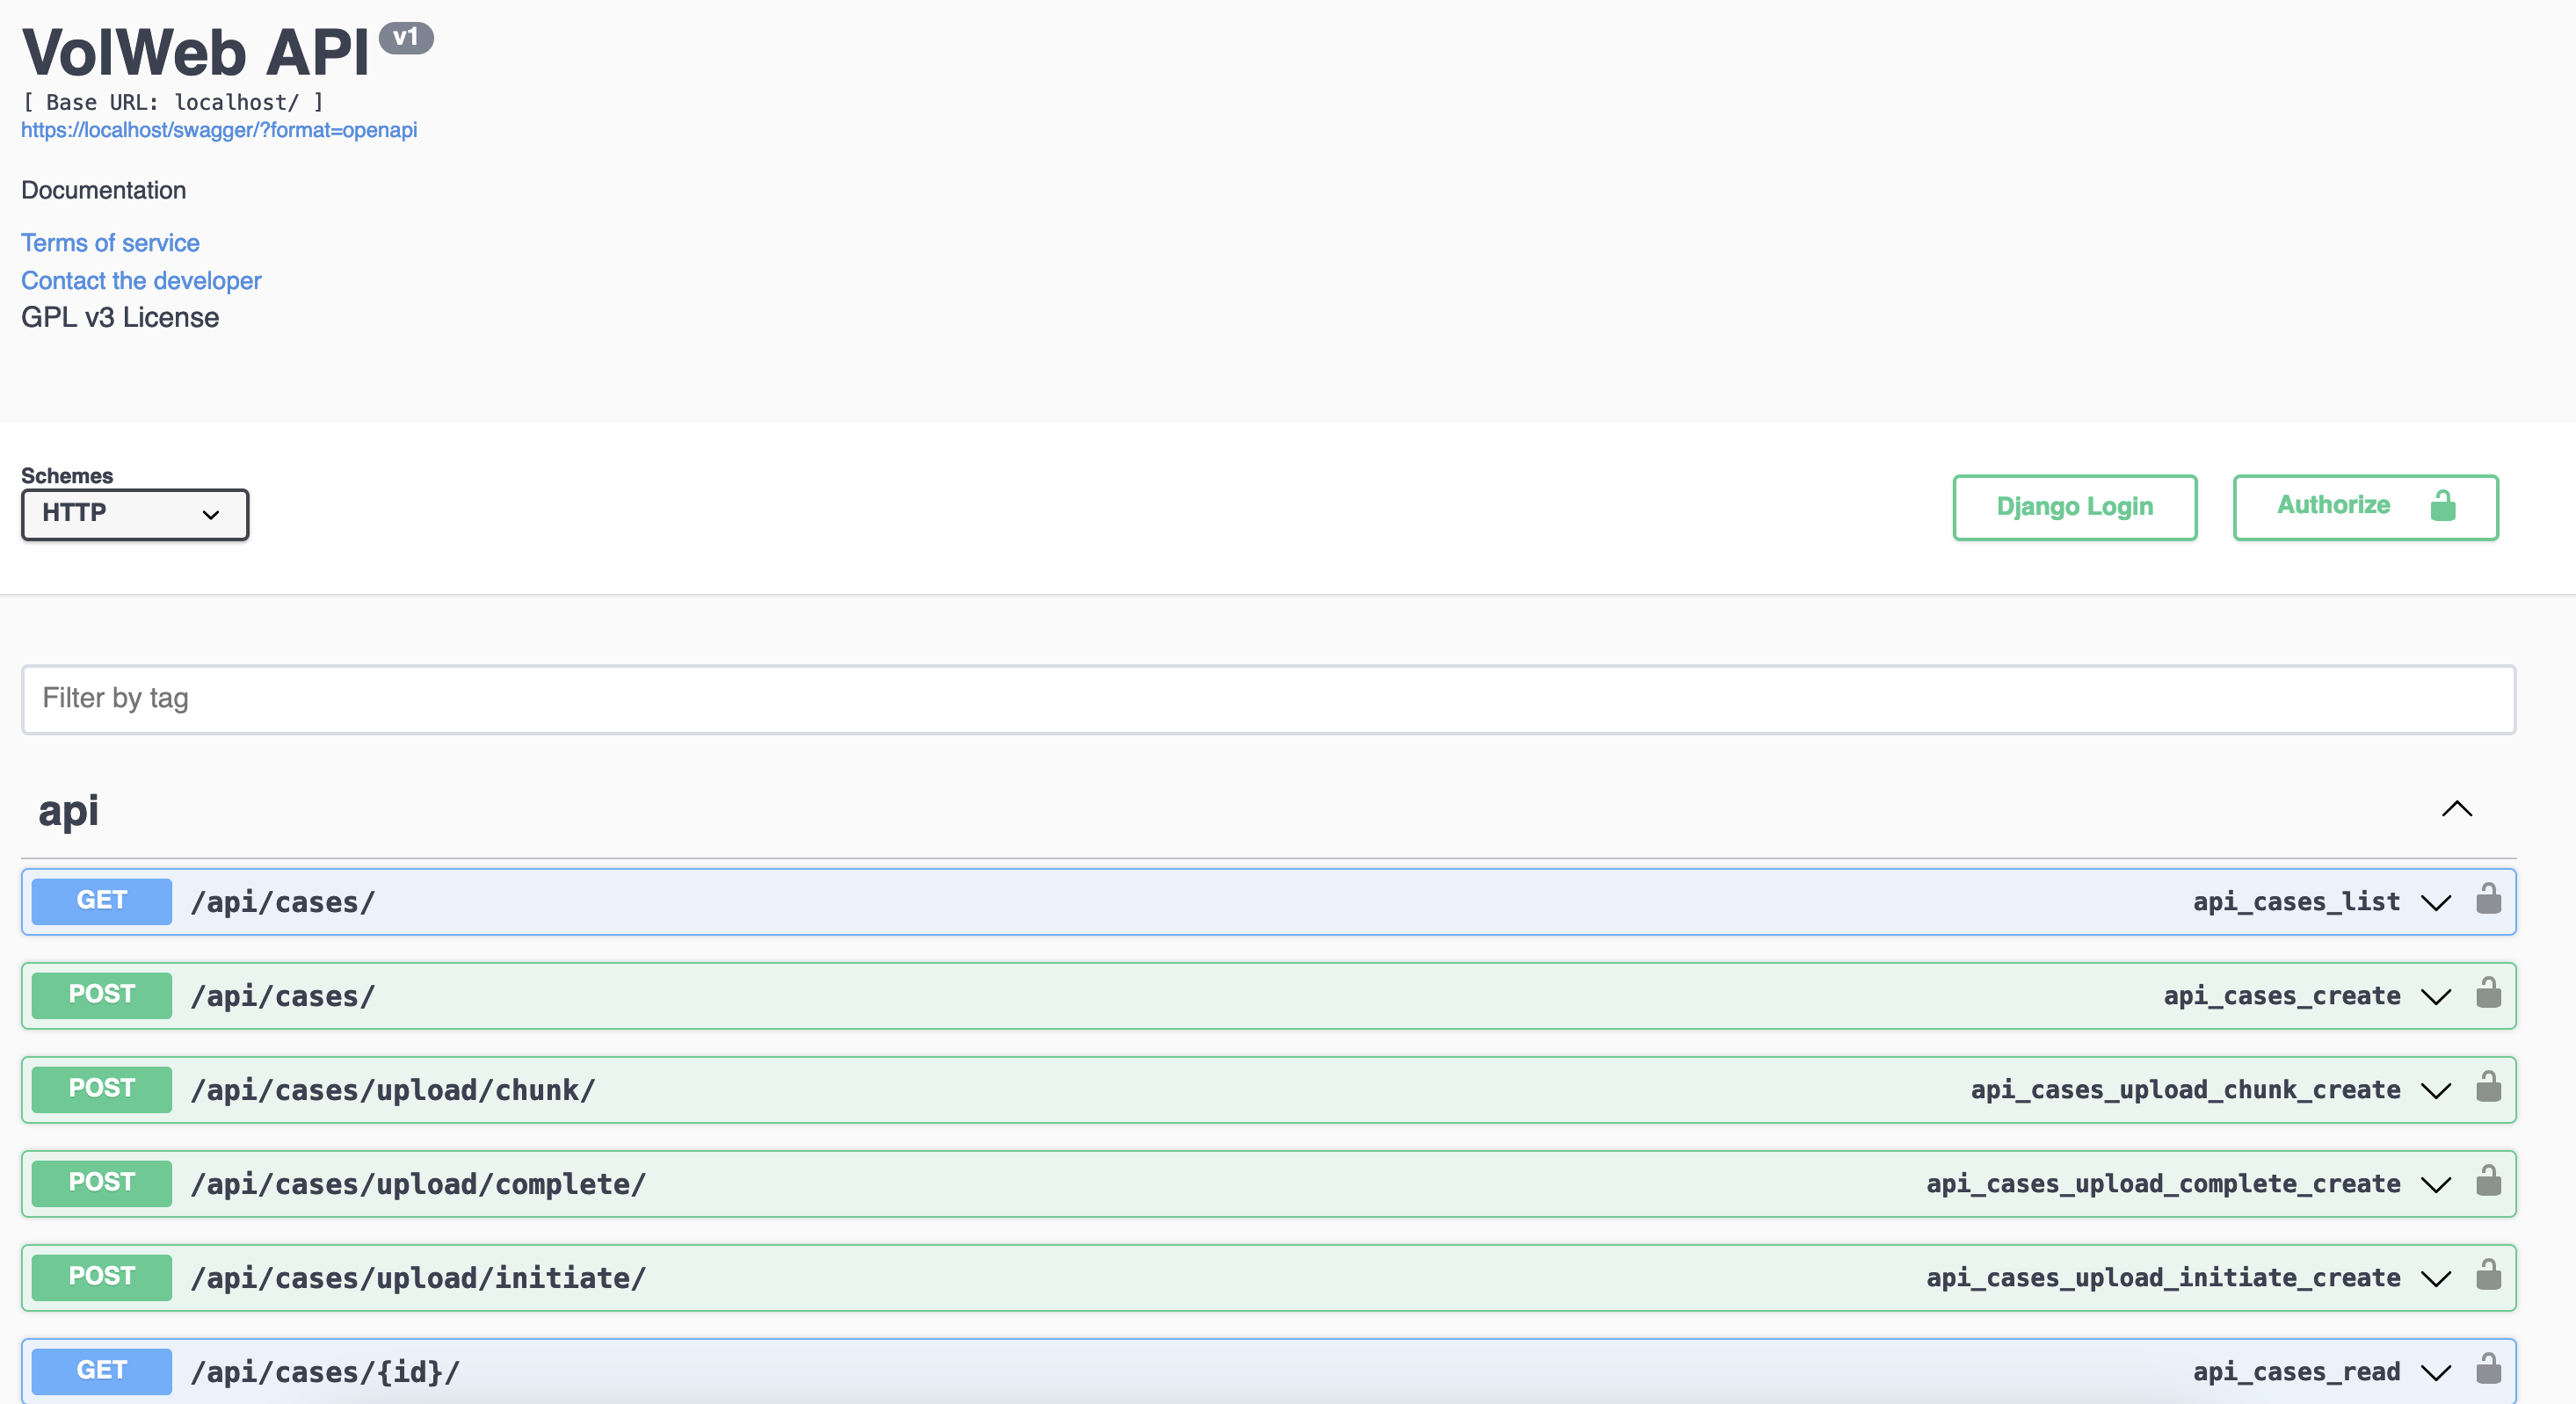
\includegraphics[width=1\linewidth]{images/volweb-original/volweb-swagger.png}
\end{figure}

\section{Gestione dei Dump di Memoria}

\subsection{Upload e storage}

La gestione di file di grandi dimensioni rappresenta una sfida tecnica significativa in un'applicazione web. I dump di memoria possono facilmente superare i 10 GB, dimensioni che mettono alla prova sia l'infrastruttura di rete che i meccanismi standard di upload HTTP. VolWeb implementa un sistema di upload chunked che divide il file in blocchi gestibili.

Il backend gestisce l'assemblaggio dei chunk e la validazione dell'integrità attraverso hash crittografici. Il sistema mantiene metadati dettagliati su ogni file, inclusi hash multipli per la verifica dell'integrità e timestamp per la chain of custody.

\subsection{Rilevamento automatico del profilo}

Uno degli aspetti più innovativi di VolWeb è il sistema di rilevamento automatico del profilo del sistema operativo. Questo processo, tradizionalmente manuale e soggetto a errori, viene automatizzato attraverso l'analisi delle strutture dati presenti nel dump. Il sistema esamina `signature` specifiche che identificano univocamente versioni di Windows, distribuzioni Linux o altri sistemi operativi supportati.

Prima vengono cercate 'signature' ad alta confidenza che permettono l'identificazione immediata. Se queste non producono risultati, il sistema procede con euristiche più complesse che analizzano pattern di strutture dati. Come fallback finale, l'utente può specificare manualmente il profilo, ma nella pratica questo è raramente necessario.

\section{Sicurezza e Controllo degli Accessi}

La sicurezza in VolWeb è implementata a più livelli, partendo da un robusto sistema di autenticazione basato sul framework di Django. Gli utenti devono autenticarsi per accedere a qualsiasi funzionalità, e le sessioni sono gestite in modo sicuro con token che scadono dopo un periodo di inattività configurabile.

Il sistema di autorizzazione implementa un modello di permessi granulare. Gli utenti possono avere ruoli diversi con capacità appropriate. A livello di caso, è possibile definire permessi specifici, permettendo la condivisione selettiva di investigazioni tra team diversi mantenendo la segregazione di informazioni sensibili.

\section{Deployment e Operazioni}
\subsection{Containerizzazione e Docker}
VolWeb fornisce una configurazione Docker completa che semplifica significativamente il deployment. Il docker-compose.yml definisce tutti i servizi necessari: web application, database, Redis e Celery workers. Questa configurazione permette di avere un ambiente completamente funzionale con un singolo comando, eliminando le complessità tipiche del setup di applicazioni multi-componente.

La containerizzazione offre vantaggi significativi per la riproducibilità e la portabilità. Gli stessi container possono essere deployati in ambiente di sviluppo, test e produzione con la garanzia di comportamento consistente. Inoltre, l'isolamento fornito dai container migliora la sicurezza, limitando l'impatto di eventuali compromissioni.

\subsection{Monitoraggio e logging}
Un sistema di logging comprensivo è fondamentale per troubleshooting e audit. VolWeb implementa logging strutturato a tutti i livelli dell'applicazione. Le azioni degli utenti sono loggate per audit trail, mentre gli errori tecnici sono catturati con contesto sufficiente per debugging. 
\begin{figure}[H]
\centering
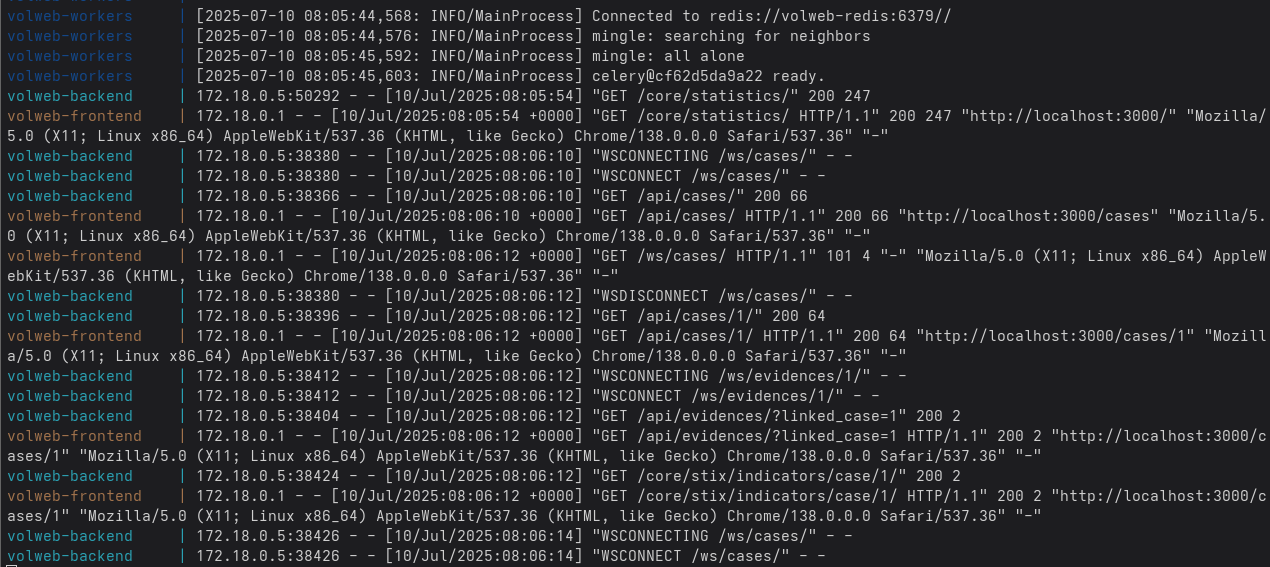
\includegraphics[width=1\linewidth]{images/volweb-original/volweb-logs.png}
\end{figure}

\section{Troubleshooting e Problemi Comuni}
\subsection{Problemi di installazione}
La wiki del progetto documenta i problemi più comuni riscontrati durante l'installazione e le relative soluzioni. Un problema frequente riguarda i permessi Docker su sistemi Linux, che può essere risolto aggiungendo l'utente al gruppo docker o eseguendo i comandi con sudo.
Conflitti di porte sono un altro problema comune, specialmente in ambienti di sviluppo dove altre applicazioni potrebbero utilizzare le porte 8000 (Django) o 6379 (Redis). La soluzione consiste nel modificare il file docker-compose.yml per utilizzare porte alternative.
Problemi di memoria durante l'analisi di dump molto grandi possono essere mitigati aumentando i limiti di memoria per i container Docker o configurando swap aggiuntivo sul sistema host.

\subsection{Problemi operativi}
Durante l'uso operativo, gli utenti potrebbero incontrare timeout durante l'upload di file molto grandi. Questo può essere risolto aumentando i timeout di nginx o del reverse proxy utilizzato. La wiki fornisce configurazioni esempio per i proxy più comuni.
Errori di analisi con specifici plugin Volatility sono spesso dovuti a incompatibilità tra il profilo del sistema operativo e il plugin. VolWeb cerca di prevenire questi errori mostrando solo plugin compatibili, ma in casi edge potrebbe essere necessario aggiornare i simboli o utilizzare plugin alternativi.

\section{Community e Contribuzioni}
\subsection{Struttura del progetto open source}
VolWeb è sviluppato come progetto open source su GitHub, accogliendo contribuzioni dalla community. Il repository segue best practice standard con branch protetti, pull request review e continuous integration. La struttura del codice è organizzata per facilitare la comprensione e le contribuzioni esterne.
Il progetto mantiene una roadmap pubblica che delinea le feature pianificate e permette alla community di contribuire con suggerimenti e prioritizzazioni. Issues e discussions su GitHub forniscono canali per supporto, bug reporting e proposte di miglioramento.
\subsection{Come contribuire}
La wiki fornisce linee guida dettagliate per chi desidera contribuire al progetto. Le contribuzioni possono assumere molte forme: sviluppo di nuove feature, fix di bug, miglioramenti alla documentazione, traduzioni dell'interfaccia, o semplicemente testing e feedback.
Per contribuzioni di codice, il processo prevede il fork del repository, lo sviluppo in un branch dedicato, e la sottomissione di una pull request con descrizione dettagliata delle modifiche. Il codice deve seguire gli standard di stile del progetto e includere test appropriati.
Contribuzioni non tecniche sono ugualmente valorizzate. Miglioramenti alla documentazione, tutorial, case study di utilizzo reale, o semplicemente la segnalazione di problemi attraverso issue ben documentate sono tutti modi validi per supportare il progetto.

\section{Casi d'Uso e Scenari Applicativi}
\subsection{Incident Response}
Nell'ambito dell'incident response, VolWeb si dimostra particolarmente efficace per l'analisi rapida di endpoint potenzialmente compromessi. Uno scenario tipico vede il team di sicurezza acquisire dump di memoria da sistemi sospetti e caricarli in VolWeb per analisi parallela. La capacità di processare più evidenze contemporaneamente permette di identificare rapidamente pattern comuni tra sistemi compromessi.
La visualizzazione interattiva dei risultati facilita l'identificazione di indicatori di compromissione come processi anomali, connessioni di rete sospette, o DLL iniettate. L'export automatico di IOC permette di alimentare rapidamente sistemi di difesa perimetrale con intelligence actionable.

\subsection{Forensics investigations}
Per investigazioni forensi più approfondite, VolWeb fornisce un ambiente strutturato per l'analisi metodica. La gestione dei casi permette di organizzare evidenze correlate, mantenere note e osservazioni, e produrre report per uso legale. La chain of custody integrata garantisce l'ammissibilità delle evidenze in contesti giudiziari.
L'accesso multi-utente con permessi granulari facilita la collaborazione tra investigatori, permettendo peer review e validazione incrociata dei findings. La persistenza completa dei risultati permette di rivisitare analisi precedenti quando emergono nuove informazioni o tecniche.

\subsection{Threat hunting}
Sebbene limitato dall'assenza di supporto YARA nella versione originale, VolWeb può comunque essere utilizzato per attività di threat hunting. L'analisi di dump da sistemi apparentemente non compromessi può rivelare attività malevole sofisticate che evadono i controlli tradizionali.
La capacità di ricerca full-text sui risultati permette di cercare artefatti specifici associati a famiglie di malware conosciute. L'analisi comparativa di dump multipli può rivelare pattern di comportamento anomalo anche in assenza di indicatori specifici.


\section{Limitazioni e Considerazioni}
\subsection{Limitazioni funzionali}
Nonostante le capacità significative, la versione originale di VolWeb presenta alcune limitazioni importanti. L'assenza di supporto per YARA rappresenta probabilmente la mancanza più significativa, limitando le capacità di threat hunting della piattaforma.
La correlazione automatica tra risultati di plugin diversi è ancora basica. Mentre VolWeb presenta i risultati in modo organizzato, manca di capacità avanzate di correlation engine che potrebbero identificare automaticamente pattern sospetti attraverso dataset diversi. Questa limitazione richiede che l'analista mantenga mentalmente le correlazioni, aumentando il carico cognitivo.
L'integrazione con threat intelligence esterna è assente. In un panorama dove la condivisione di IOC e intelligence è fondamentale, l'impossibilità di importare automaticamente feed di threat intelligence o di arricchire i risultati con contesto esterno rappresenta una limitazione operativa significativa.

\subsection{Scalabilità e performance}
Mentre VolWeb gestisce efficacemente dump di dimensioni moderate, l'analisi di dump molto grandi (>32GB) o l'analisi simultanea di molti dump può mettere alla prova l'architettura. La natura single-threaded di alcuni componenti di Volatility limita la parallelizzazione, creando colli di bottiglia in scenari di alto carico.
La gestione dello storage può diventare problematica in deployment di grandi dimensioni. Senza meccanismi automatici di archiviazione o tiering, lo storage dei dump può rapidamente consumare spazio disco significativo. Organizzazioni con requisiti di retention lunghi devono implementare soluzioni custom per la gestione del ciclo di vita dei dati.

\subsection{Roadmap futura}
La documentazione del progetto delinea una roadmap ambiziosa per il futuro di VolWeb. Le priorità immediate includono l'integrazione di YARA per capacità di pattern matching avanzate, il miglioramento delle visualizzazioni con timeline correlate e grafi interattivi più sofisticati, e l'implementazione di un sistema di reporting automatico per generazione di documenti professionali.
Nel medio termine, il progetto punta all'integrazione con piattaforme di threat intelligence per arricchimento automatico dei dati, all'implementazione di capacità di machine learning per anomaly detection, e al supporto per analisi di memoria da container e ambienti virtualizzati.
La visione a lungo termine include l'evoluzione verso una piattaforma di analisi forense completa che integri memoria, disco e network forensics in un'unica interfaccia coerente, supportando workflow investigativi end-to-end.


\section{Conclusioni}
VolWeb rappresenta un contributo significativo all'ecosistema della memory forensics, abbassando drasticamente la barriera all'ingresso per l'utilizzo di Volatility. L'architettura moderna, l'interfaccia intuitiva e l'automazione di task complessi lo rendono uno strumento prezioso per team di sicurezza di ogni dimensione.
L'approccio open source e l'architettura modulare hanno creato una base solida per future espansioni. La community ha già dimostrato interesse nel progetto, contribuendo bug fix e suggerimenti per miglioramenti. Questo engagement della community è fondamentale per l'evoluzione continua della piattaforma.
Tuttavia, le limitazioni identificate, in particolare l'assenza di supporto YARA, rappresentano ostacoli significativi per l'adozione in contesti enterprise avanzati. Queste limitazioni non sono mere mancanze di feature, ma gap funzionali che limitano l'efficacia operativa della piattaforma in scenari reali di incident response e threat hunting.